%!TEX root = ../../main.tex
\section{APPLICATIONS OF ANOMALY DETECTION}
\label{sec:applicationsOfDLAD}



In this section we discuss several applications of anomaly detection. For each application
domain we discuss the following four aspects:\\
\textemdash the notion of anomaly;\\
\textemdash nature of the data;\\
\textemdash challenges associated with detecting anomalies;\\
\textemdash existing anomaly detection techniques.\\

% %!TEX root = ../../main.tex
\subsection{Intrusion Detection}
\label{sec:intrusion_detection}

Intrusion detection  system (IDS) refers to identifying malicious activity in a computer related system~\cite{phoha2002internet}. IDS may be deployed at single computers known as Host Intrusion Detection (HIDS) to large networks Network Intrusion Detection (NIDS). The classification of deep anomaly detection techniques for intrusion detection is in Figure ~\ref{fig:deepADforIDS}. IDS depending on detection method are classified into signature based or anomaly based. Using signature based IDS is not efficient to detect new attacks, for which no specific signature pattern is available, hence anomaly based detection methods are more popular. In this survey we focus on deep anomaly detection (DAD) methods and architectures employed in intrusion detection.
\vspace{-0.3cm}
\subsubsection{Host-Based Intrusion Detection Systems (HIDS):}
 Such systems are installed software programs which monitors a single host or computer for malicious  activity or policy violations by listening to system calls or events occurring within that host ~\cite{vigna2005host}. The system call logs could be generated by programs or by user interaction resulting in logs as shown in Figure ~\ref{fig:syslog}. Malicious interactions lead to execution of these system calls in different sequences. HIDS may also monitor the state of a system, its stored information, in Random Access Memory (RAM), in the file system, log files or elsewhere for a valid sequence.
 Deep anomaly detection (DAD) techniques applied for HIDS are required to handle the variable length and sequential nature of data. The DAD techniques have to either model the sequence data or compute similarity between sequences. Some of the success-full DAD techniques for HIDS is illustrated in Table~\ref{tab:HIDS}.

\subsubsection{Network Intrusion Detection Systems (NIDS):} NIDS systems deal with monitoring the entire network for suspicious traffic by examining each and every network packet. Owing to real-time streaming behaviour, the nature of data is synonymous to big data with high volume, velocity, variety. The network data also has a temporal aspect associated with it. Some of the success-full DAD techniques for NIDS is illustrated in Table~\ref{tab:NIDS}. This survey also lists the data-sets used for evaluating the DAD intrusion detection methods in Table~\ref{tab:IDSDataset}. A challenge faced by DAD techniques in intrusion detection is that the nature of anomalies keeps changing over time as the intruders adapt their network attacks to evade the existing intrusion detection solutions.

% Begin Figure
\begin{figure*}
\centering
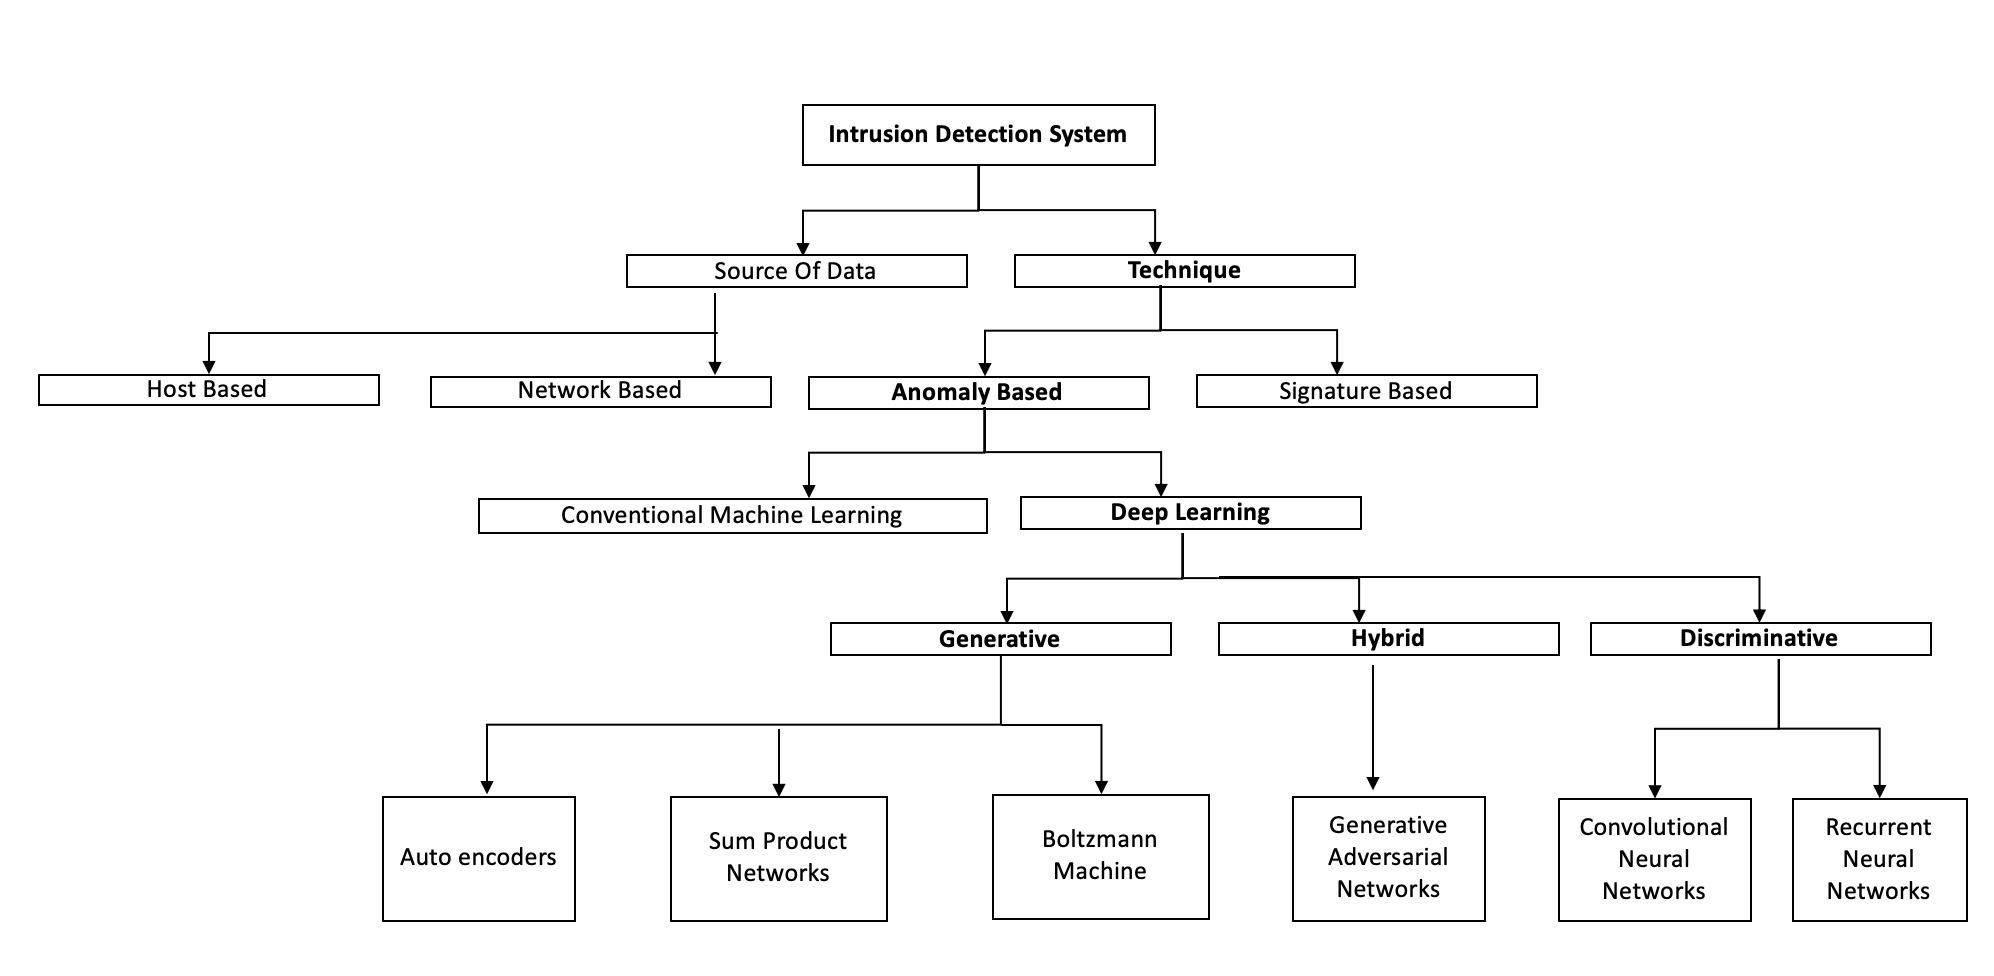
\includegraphics[scale=0.4]{images/IDS}
\captionsetup{justification=centering}
\caption{Classification of deep learning methods for intrusion detection.}
\label{fig:deepADforIDS}
\end{figure*}
% End of Figure


%%%%%%% HIDS Network intrusion detection%%%%%%%
%%% Table  Describing the model architectures and techniques used  of HIDS
\begin{table}
\begin{center}
\caption{Examples of DAD Techniques employed in HIDS
          \\CNN: Convolution Neural Networks, LSTM : Long Short Term Memory Networks
          \\GRU: Gated Recurrent Unit, DNN : Deep Neural Networks
          \\SPN: Sum Product Networks}
 \captionsetup{justification=centering}
  \label{tab:HIDS}
   \scalebox{0.82}{
    \begin{tabular}{ | l | p{4cm} | l | p{5cm} |}
    \hline
    Techniques & Model Architecture & Section & References \\ \hline
    Discriminative &  LSTM , CNN-LSTM-GRU, DNN & Section ~\ref{sec:rnn_lstm_gru},~\ref{sec:cnn},~\ref{sec:dnn} &  \cite{kim2016lstm},\cite{chawla2018host},\cite{chen2018henet},\cite{sohi2018recurrent},\cite{vinayakumar2017applying} \\\hline
    Hybrid &  GAN & Section ~\ref{sec:hybridModels} & \cite{aghakhani2018detecting}, \cite{li2018anomaly} \\\hline
    Generative &  AE, SPN,  & Section ~\ref{sec:ae},~\ref{sec:spn} & \cite{gao2014intrusion},\cite{peharz2018probabilistic},\cite{umer2018two} \\
    \hline
    \end{tabular}}
\end{center}
\end{table}
%%%% End of Table NIDS




%%% Host based Intrusion detection system table%%%%%%
%%% Table  Describing the model architectures and techniques used  of NIDS
\begin{table}
\begin{center}
  \caption{Examples of DAD Techniques employed in NIDS.
          \\CNN: Convolution Neural Networks, LSTM : Long Short Term Memory Networks
          \\RNN: Recurrent Neural Networks, RBM : Restricted Boltzmann Machines
          \\DCA: Dilated Convolution Autoencoders, DBN : Deep Belief Network
          \\AE: Autoencoders, SAE: Stacked Autoencoders
          \\GAN: Generative Adversarial Networks, CVAE : Convolutional Variational Autoencoder. }
  \captionsetup{justification=centering}

  \label{tab:NIDS}
  \scalebox{0.80}{
    \begin{tabular}{ | l | p{4cm} | p{5cm}  | p{7cm} |}
    \hline
    Techniques & Model Architecture & Section & References \\ \hline
   Generative  & DCA, SAE, RBM, DBN, CVAE & Section ~\ref{sec:cnn},~\ref{sec:ae},~\ref{sec:dnn},~\ref{sec:gan_adversarial} & \cite{yu2017network},\cite{thing2017ieee}, \cite{zolotukhin2016increasing},~\cite{cordero2016analyzing},\cite{alrawashdeh2016toward},\cite{tang2016deep},\cite{lopez2017conditional},\cite{al2018deep},\cite{mirsky2018kitsune},\cite{aygun2017network} \\ \hline
  Hybrid  & GAN   & Section ~\ref{sec:hybridModels} & \cite{lin2018idsgan},\cite{yin2018enhancing}, \cite{ring2018flow}, \cite{latah2018deep},\cite{intrator2018mdgan},\cite{matsubara2018anomaly},~\cite{nicolau2016hybrid} ,\cite{rigaki2017adversarial}. \\ \hline
  Discriminative &  RNN , LSTM ,CNN & Section ~\ref{sec:rnn_lstm_gru},~\ref{sec:cnn} & \cite{yu2017network}, \cite{malaiya2018empirical} \cite{kwon2018empirical},\cite{gao2014intrusion},\cite{staudemeyer2015applying},\cite{naseer2018enhanced}\\
  \hline
  \end{tabular}}
\end{center}
\end{table}
%%%% End of Table NIDS


% Datasets Used Table
%%% Host based Intrusion detection system table%%%%%%
%%% Table  Describing the model architectures and techniques used  of NIDS
\begin{table*}
\begin{center}
  \caption{Datasets Used in Intrusion Detection }
   \label{tab:IDSDataset}
    \scalebox{0.85}{
    \begin{tabular}{ | p{3cm} | l | p{5cm} | p{3cm} | p{5cm} |}
    \hline
    DataSet &IDS & Description & Type & References \\ \hline
    CTU-UNB & NIDS & CTU-UNB~\cite{ucsdAnomalyDetect2017} dataset consists of various botnet traffics from CTU-13 dataset [20] and normal traffics from the UNB ISCX IDS 2012 dataset ~\cite{shiravi2012toward}  & Hexadecimal & \cite{yu2017network} \\ \hline
    Contagio-CTU-UNB & NIDS  & Contagio-CTU-UNB dataset consists of six types of network traffic data. ~\cite{adam2008robust}  & Text & ~\cite{yu2017network}. \\ \hline
    NSL-KDD~\footnote{http://nsl.cs.unb.ca/NSL-KDD/}& NIDS &The NSL-KDD data set is a refined version of its predecessor KDD-99 data set.  ~\cite{ucsdAnomalyDetect2017} & Text &  ~\cite{yin2017deep},~\cite{javaid2016deep},  ~\cite{tang2016deep},~\cite{yousefi2017autoencoder},~\cite{mohammadi2017new}, ~\cite{lopez2017conditional}\\\hline
    DARPA KDD- CUP 99 & NIDS & DARPA KDD~\cite{stolfo2000cost} The competition task was to build a network intrusion detector, a predictive model capable of distinguishing between ``bad'' connections, called intrusions or attacks, and ``good'' normal connections.  & Text   & ~\cite{alrawashdeh2016toward} ,~\cite{van2017anomaly},~\cite{mohammadi2017new}\\\hline
    MAWI& NIDS  & The  MAWI~\cite{fontugne2010mawilab}  dataset  consists  of  network  traffic  capturedfrom  backbone  links  between  Japan  and  USA.  Every  daysince  2007  & Text   & ~\cite{cordero2016analyzing} \\\hline
    Realistic Global Cyber Environment (RGCE) & NIDS & RGCE~\cite{jamkRGCE}  contains
    realistic Internet Service Providers (ISPs) and numerous different web services as
    in the real Internet.  &  Text   & ~\cite{zolotukhin2016increasing} \\\hline
    ADFA-LD& HIDS & The ADFA Linux Dataset (ADFA-LD). This dataset provides a contemporary Linux dataset for evaluation by traditional HIDS~\cite{creech2014semantic} & Text   & ~\cite{kim2016lstm},~\cite{chawla2018host} \\\hline
    UNM-LPR& HIDS & Consists of system calls to evalute HIDS system~\cite{ImmuneDatasets} & Text   & ~\cite{kim2016lstm} \\\hline
    Infected PDF samples& HIDS & Consists of set of Infected PDF samples, which are used to monitor the malicious traffic  & Text   &~\cite{chen2018henet}\\\hline
    \end{tabular}}
\end{center}
\end{table*}
%%%% End of Table NIDS













% \label{sec:intrusionDetect}

%!TEX root = ../../main.tex
\subsection{Malware Detection}
\label{sec:malwaredetection}

Malware, short for Malicious Software. In  order to protect legitimate users from malware, machine learning based efficient malware detection methods are proposed~\cite{ye2017survey}. In the classical machine learning methods, the process of malware detection is usually divided into two stages: feature extraction and classification/clustering. The performance of traditional malware detection approaches critically depend on the extracted features and the methods for classification/clustering. The challenge associated in malware detection problems is the seer scale of data, for instance considering data as bytes a certain  sequence classification problem could be  of the order of two million time steps. Furthermore the malware is very adpative in nature, wherein the attackers would use advanced techniques to hide the malicious behaviour. Some DAD techniques  which address these challenges effectively and detect malware are shown in Table~\ref{tab:malwareDetect}.

\begin{table*}
  \begin{center}
   \caption{Examples of DAD techniques used for malware detection.
             \\AE: Autoencoders, LSTM : Long Short Term Memory Networks
             \\RBM: Restricted Botlzmann Machines, DNN : Deep Neural Networks
             \\GRU: Gated Recurrent Unit, RNN: Recurrent Neural Networks
             \\CNN: Convolutional Neural Networks,VAE: Variational Autoencoders
             \\GAN: Generative Adversarial Networks,CNN-BiLSTM: CNN- Bidirectional LSTM}
    \captionsetup{justification=centering}
    \label{tab:malwareDetect}
    \scalebox{0.85}{
    \begin{tabular}{|p{3cm}|p{2cm}|p{10cm}|}
      \hline
      \textbf{Technique Used} & \textbf{Section} & \textbf{References}\\
      \hline
      AE &  Section ~\ref{sec:ae}  & ~\cite{yousefi2017autoencoder},~\cite{hardy2016dl4md},~\cite{yousefi2017autoencoder},~\cite{de2018malware},~\cite{sewak2018investigation},~\cite{kebede2017classification},~\cite{de2018malware},~\cite{david2015deepsign}\\\hline
      word2vec & Section ~\ref{sec:word2vec} &  ~\cite{cakir2018malware},~\cite{silva2018improving}\\\hline
      CNN & Section ~\ref{sec:cnn} &  ~\cite{kolosnjaji2018adversarial},~\cite{suciu2018exploring},~\cite{srisakaokul2018muldef},~\cite{srisakaokul2018muldef},~\cite{king2018artificial},~\cite{huang2017r2},~\cite{guo2017malware},~\cite{abdelsalam2018malware},\newline ~\cite{raff2017malware},~\cite{karbab2018maldozer},~\cite{martinelli2017evaluating},~\cite{mclaughlin2017deep},~\cite{gibert2018using},~\cite{kolosnjaji2017empowering}\\\hline
      DNN & Section ~\ref{sec:dnn} &  ~\cite{rosenberg2018end},~\cite{wang2017adversary}\\\hline
      DBN & Section ~\ref{sec:dnn} &  ~\cite{david2015deepsign},~\cite{yang2016application},~\cite{ding2016application},~\cite{yuxin2017malware},~\cite{selvaganapathy2018deep},~\cite{yuxin2017malware},~\cite{hou2017deep}\\\hline
      LSTM & Section ~\ref{sec:rnn_lstm_gru} &  ~\cite{tobiyama2016malware}, ~\cite{hu2017black},~\cite{tobiyama2018method} ,~\cite{passalislong} \\\hline
      CNN-BiLSTM& Section ~\ref{sec:cnn},~\ref{sec:rnn_lstm_gru} &  ~\cite{le2018deep},~\cite{wang2017adversary} \\\hline
      GAN& Section ~\ref{sec:gan_adversarial} &  ~\cite{kim2018zero} \\\hline
      Hybrid model(AE-CNN),(AE-DBN) & Section ~\ref{sec:hybridModels} &  ~\cite{wang2018effective},~\cite{li2015hybrid} \\\hline
      RNN & Section ~\ref{sec:rnn_lstm_gru} &  ~\cite{haddadpajouh2018deep} \\\hline
    \end{tabular}}
  \end{center}
\end{table*}



% OCSVM~\cite{scholkopf2002support}, SVDD~\cite{scholkopf2002support}
% SVM~\cite{cortes1995support}
% KNN~\cite{altman1992introduction}
% Random Forest~\cite{ho1995random}
% Relief~\cite{kira1992feature}
% CSI~\cite{ruchansky2017csi}
% \ref{sec:dnn}
% \ref{sec:stn}
% \ref{sec:spn}
% \ref{sec:word2vec}
% \ref{sec:gan_adversarial}
% \ref{sec:cnn}
% \ref{sec:rnn_lstm_gru}
% \ref{sec:ae}





\label{sec:malwareDetection}

%!TEX root = ../../main.tex
\subsection{Industrial Anomalies Detection}

Industrial systems consisting of wind turbines, power plants, high-temperature energy systems, storage devices and  with rotating mechanical parts are exposed to enormous stress on a day-to-day basis. Damage to these type of systems not only causes economic loss but also a loss of reputation, therefore detecting and repairing them early is of utmost importance. Several machine learning techniques have been used to detect such damage in industrial systems ~\cite{ramotsoela2018survey,marti2015anomaly}. Several papers published utilizing deep learning models for detecting early industrial damage show great promise~\cite{atha2018evaluation,de2018automatic,wang2018residential}. Damages caused to equipment's are rare events, thus  detecting such events can be formulated as outlier detection problem. The challenges associated with outlier detection in this domain is both volume as well as dynamic nature of data, since failure can be caused due to variety of factors. Some of the DAD techniques employed across various industries are illustrated in Table ~\ref{tab:industrialDamageDetect}.



%%%%%%% Begin table industrial damage detection
\begin{table*}
\begin{center}
\caption{Examples of DAD techniques used in industrial operations.
        \\CNN: Convolution Neural Networks, LSTM : Long Short Term Memory Networks
        \\GRU: Gated Recurrent Unit, DNN : Deep Neural Networks
        \\AE: Autoencoders, DAE: Denoising Autoencoders, SVM: Support Vector Machines
        \\SDAE: Stacked Denoising Autoencoders, RNN : Recurrent Neural Networks.}
    \label{tab:industrialDamageDetect}
    \captionsetup{justification=centering}
    \scalebox{0.85}{
    \begin{tabular}{ | l | p{2cm} | p{8cm} |}
    \hline
     \textbf{Techniques}  & \textbf{Section} & \textbf{References} \\ \hline
     LSTM & Section ~\ref{sec:rnn_lstm_gru} &  ~\cite{inoue2017anomaly},~\cite{thi2017one},~\cite{kravchik2018detecting},~\cite{huang2018deep},~\cite{park2018lired},~\cite{chang2018review}\\\hline
     AE & Section ~\ref{sec:ae} & ~\cite{yuan2015distributed},~\cite{araya2017ensemble},~\cite{qu2017detection},~\cite{sakurada2014anomaly},~\cite{bhattad2018detecting}\\\hline
     DNN & Section ~\ref{sec:dnn} & ~\cite{lodhi2017power}\\\hline
     CNN & Section ~\ref{sec:cnn} & ~\cite{faghih2016deep},~\cite{christiansen2016deepanomaly},~\cite{lee2016convolutional},~\cite{faghih2016deep}, ~\cite{dong2016camera},~\cite{nanduri2016anomaly},~\cite{fuentes2017robust},~\cite{huang2018deep},~\cite{chang2018review}\\\hline
     SDAE,DAE & Section ~\ref{sec:ae} & ~\cite{yan2015accurate},~\cite{luo2017gas},~\cite{dai2017cleaning} \\\hline
     RNN & Section ~\ref{sec:rnn_lstm_gru} & ~\cite{banjanovic2017neural},~\cite{thi2017one} \\\hline
     Hybrid Models (DNN-SVM) & Section ~\ref{sec:hybridModels} & ~\cite{inoue2017anomaly} \\\hline
    \end{tabular}}
\end{center}
\end{table*}
%%%%%%%%% End of industrial damage detection












\label{sec:industrialDamageDetect}


%!TEX root = ../../main.tex

%%%%%%% Begin table for video survellienace anomaly detection
\begin{table*}
\begin{center}
\caption{Examples of DAD techniques used in video surveillance.
        \\CNN: Convolution Neural Networks, LSTM : Long Short Term Memory Networks
        \\RBM: Restricted Boltzmann Machine, DNN : Deep Neural Networks
        \\AE: Autoencoders, DAE: Denoising Autoencoders
        \\OCSVM: One class Support vector machines, CAE: Convolutional Autoencoders
        \\SDAE: Stacked Denoising Autoencoders, STN : Spatial Transformer Networks }
  \label{tab:videoSurvellianceAnomalyDetect}
  \captionsetup{justification=centering}
  \scalebox{0.80}{
    \begin{tabular}{ | p{3cm} | p{4cm} | p{12cm} |}
      \hline
      \textbf{Technique Used} & \textbf{Section} & \textbf{References}\\
      \hline
      CNN & Section ~\ref{sec:cnn} & \cite{dong2016camera},\cite{andrewsaanomaly},\cite{sabokrou2016fully},\cite{sabokrou2017deep},\cite{munawar2017spatio},\cite{li2017transferred},\cite{qiao2017abnormal},\cite{tripathi2018convolutional},\cite{nogas2018deepfall},\cite{christiansen2016deepanomaly},\cite{li2017transferred}\\\hline
      SAE (AE-CNN-LSTM)  &  Section ~\ref{sec:ae},~\ref{sec:cnn},~\ref{sec:rnn_lstm_gru}  & ~\cite{chong2017abnormal},~\cite{qiao2017abnormal},~\cite{khaleghi2018improved}\\\hline
      AE &  Section ~\ref{sec:ae}  & \cite{qiao2017abnormal},\cite{yang2015unsupervised},\cite{chen2015detecting},\cite{gutoskidetection},\cite{d2017autoencoder},\cite{dotti2017unsupervised},\cite{yang2015unsupervised},\cite{chen2015detecting},\cite{sabokrou2016video},\cite{tran2017anomaly},\cite{chen2015detecting} ,\cite{d2017autoencoder},\cite{hasan2016learning},\cite{yang2015unsupervised},\cite{cinelli2017anomaly}\\\hline
      Hybrid Model (CAE-OCSVM) & Section ~\ref{sec:hybridModels}  & ~\cite{gutoskidetection}, ~\cite{dotti2017unsupervised}\\\hline
      LSTM-AE &  Section ~\ref{sec:rnn_lstm_gru}, ~\ref{sec:ae}  & ~\cite{d2017autoencoder}\\\hline
      STN &Section~\ref{sec:stn}   & \cite{chianucci2016unsupervised}\\\hline
      RBM &Section ~\ref{sec:dnn}   & \cite{munawar2017spatio}\\\hline
      LSTM &Section ~\ref{sec:rnn_lstm_gru}  &~\cite{medel2016anomaly},~\cite{luo2017remembering},~\cite{ben2018attentioned},~\cite{singh2017anomaly}\\\hline
      RNN & Section ~\ref{sec:rnn_lstm_gru} &\cite{luo2017revisit},\cite{zhou2015abnormal} ,\cite{hu2016video},~\cite{chong2015modeling}\\\hline
      AAE & Section ~\ref{sec:gan_adversarial} & ~\cite{ravanbakhsh2017training}\\\hline
    \end{tabular}}
  \end{center}
\end{table*}
%%%%%%%%% End of video survellienace anomaly detection


\subsection{Video Surveillance}
Video Surveillance also popularly known as Closed-circuit television (CCTV) involves monitoring a designated areas of interest in order to ensure security. In videos surveillance applications unlabelled data is available in large amounts, this is a significant challenge for supervised machine learning and deep learning methods. Hence video surveillance applications have been modelled as anomaly detection problems owing to lack of availability of labelled data. Several works have studied the state-of-the-art deep models for video anomaly detection and  have classified them based on the type of model and criteria of detection~\cite{kiran2018overview,chong2015modeling}. The challenges of robust 24/7 video surveillance systems is discussed in detail by Boghossian et.al~\cite{boghossian2005challenges}. The lack of  explicit definition of anomaly in real-life video surveillance is a significant issue that hampers the performance of DAD methods as well. DAD techniques used in  video surveillance  are illustrated  in Table ~\ref{tab:videoSurvellianceAnomalyDetect}.







% % Datasets Used Table
% \begin{table*}
%   \begin{center}
%     \caption{Datasets Used For Video surveillance}
%     \label{tab:videoSurvelliance}
%     \begin{tabular}{|p{3cm}|p{4cm}|p{6cm}|}
%       \hline
%       \textbf{DataSet} & \textbf{Type} & \textbf{References}\\
%       \hline
%       UCSD Ped2~\cite{ucsdAnomalyDetect2017},Subway~\cite{adam2008robust} &  Video   & Sabokrou et al~\cite{sabokrou2016fully,sabokrou2017deep}, Gutoski et al~\cite{gutoskidetection} \\ \hline
%       LOST ~\cite{Abrams et al. 2012} &  Video   & Dotti et al~\cite{dotti2017unsupervised}\\ \hline
%       YouTube &  Video   & Yang et al~\cite{yang2015unsupervised}\\ \hline
%       UMN~\footnote{$http://mha.cs.umn.edu$} &  Video   & Sabokrou et al~\cite{yang2015unsupervised}\\ \hline
%       CIFAR-10 &Images& Munawar et al~\cite{munawar2017spatio} \\ \hline
%     \end{tabular}
%   \end{center}
% \end{table*}
% %%%%%%%%% End of Datasets used in video survellienace anomaly detection



































\label{sec:videoSurvelliance}


%!TEX root = ../../main.tex
\subsection{Deep learning for Anomaly detection in Social Networks}
In recent times, online social networks has become part and parcel of daily life. Anomalies in social network
are irregular often unlawful behaviour pattern of individuals within a social network, such  individuals may be identified as  spammers, sexual predators, online fraudsters, fake users or rumour-mongers. Detecting these irregular patterns is of prime importance since if not detected, the act of such individuals can have serious social impact. A survey of traditional anomaly detection techniques and its challenges to detect anomalies in social networks is a well studied topic in literature ~\cite{liu2017social,savage2014anomaly,anand2017anomaly,yu2016survey,cao2018automatic,yu2016survey}. The heterogeneous and dynamic nature of data presents significant challenges to DAD techniques. Despite these challenges several DAD techniques illustrated in Table ~\ref{tab:socialNetworkAnomalyDetect} are shown outperform state-of-the-art methods.

% Table
\begin{table*}
  \begin{center}
   \caption{Examples of DAD techniques used to detect anomalies in social network.
            \\CNN: Convolution Neural Networks, LSTM : Long Short Term Memory Networks
            \\AE: Autoencoders, DAE: Denoising Autoencoders
            \\SVM : Support Vector Machines., DNN : Deep Neural Network  }
    \captionsetup{justification=centering}
    \label{tab:socialNetworkAnomalyDetect}
    \scalebox{0.85}{
    \begin{tabular}{|p{3cm}|p{4cm}|p{5cm}|}
      \hline
      \textbf{Technique Used} & \textbf{Section} & \textbf{References}\\
      \hline
      AE,DAE &  Section ~\ref{sec:ae}  & ~\cite{zhang2017detecting},~\cite{castellini2017fake}\\\hline
      CNN-LSTM & Section ~\ref{sec:cnn}, ~\ref{sec:rnn_lstm_gru} & ~\cite{sun2018detecting},~\cite{shu2017doc},~\cite{yang2018anomaly}\\\hline
      DNN & Section ~\ref{sec:dnn}  & ~\cite{li2017detecting}\\\hline
      Hybrid Models (CNN-LSTM-SVM) & Section ~\ref{sec:hybridModels}  & ~\cite{wei2017new}\\\hline
    \end{tabular}}
  \end{center}
\end{table*}





% Science is a belief in the ingnorance of experts
% Measure of ignorance; Data Artist
% Find Worst Case: Piano
%New Ideas in Business and Intelligence and customer analytics
%Learn the rules like a professional but break like an artist

\label{sec:socialNetworks}

% %!TEX root = ../../main.tex
\subsection{Fraud Detection}
Fraud is a deliberate act of deception to access valuable resources~\cite{abdallah2016fraud}. The PwC global economic crime survey of 2018~\cite{Lavion2018,zhao2013fraud} found that half of the 7,200 companies they surveyed had experienced fraud of some nature. Fraud detection refers to detection of unlawful activities across various industries, illustrated in Figure ~\ref{fig:AerasOfFraud}.

%%%%% Figure
\begin{figure}[h]
\centering
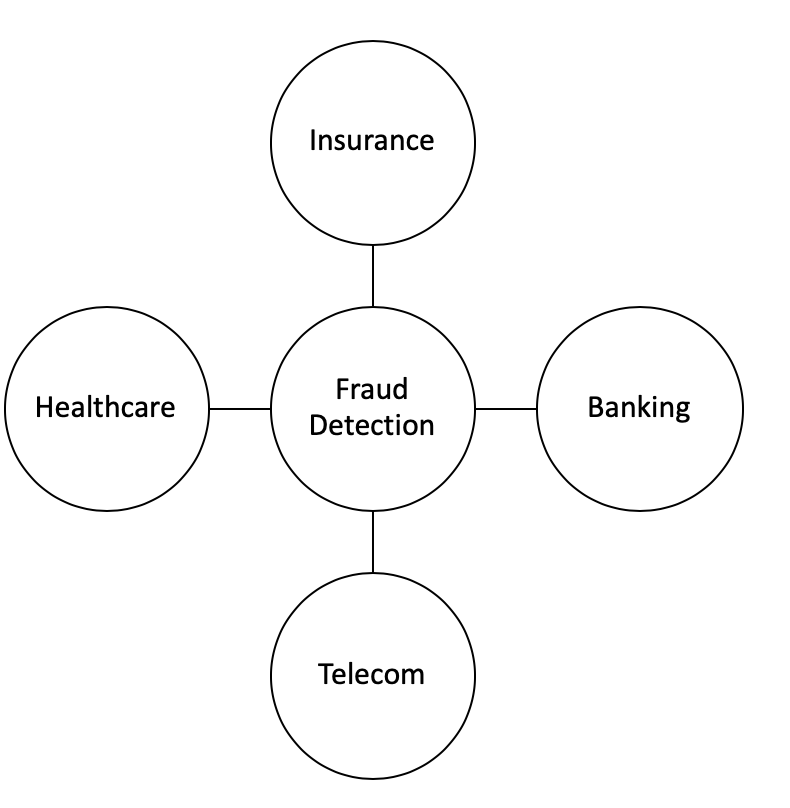
\includegraphics[scale=0.5]{images/AreasOfFraud}
\captionsetup{justification=centering}
\caption{Fraud detection across various application domains.}
\label{fig:AerasOfFraud}
\end{figure}
%%%%%%

Fraud in telecommunications, insurance \textit{( health, automobile, etc)} claims, banking \textit{( tax return claims, credit card transactions etc)} represent significant problems in both governments and private businesses. Detecting and preventing fraud is not a simple task since fraud is an adaptive crime. Many traditional machine learning algorithms have been applied successfully in fraud detection~\cite{sorournejad2016survey}.  The challenge associated with detecting fraud is that it requires real time detection and prevention. This section focuses on deep anomaly detection (DAD) techniques for fraud detection.
%-----------------------------------------------------------------------------------------------------------

\subsubsection{Banking fraud}
In the past decade, credit card was introduced in the banking sector. Now, credit card has become a popular
payment method in online shopping for goods and services. Credit card fraud involves theft of a payment card details, and use it as a fraudulent source of funds in a transaction. Many techniques for credit card fraud detection have been presented in the last few years~\cite{zhou2018state},~\cite{suganya2015survey}. We will briefly review some of DAD techniques as shown Table~\ref{tab:creditfraudDetect}.
The challenge in credit card fraud detection is that frauds have no constant patterns. The typical approach in credit card fraud detection is to maintain a usage profile for each user and monitor the user profiles to detect any deviations. Since there are billions of credit card users this technique of user profile approach is not very scalable. Owing to the inherent scalable nature of DAD techniques, these techniques are gaining wide spread adoption in credit card fraud detection.
%%%%%%% Begin table fraud detection
\begin{table*}
\begin{center}
  \caption{Examples of DAD techniques used in  credit card fraud detection.
          \\AE: Autoencoders, LSTM : Long Short Term Memory Networks
          \\RBM: Restricted Botlzmann Machines, DNN : Deep Neural Networks
          \\GRU: Gated Recurrent Unit, RNN: Recurrent Neural Networks
          \\CNN: Convolutional Neural Networks,VAE: Variational Autoencoders
          \\GAN: Generative Adversarial Networks}
  \captionsetup{justification=centering}
  \label{tab:creditfraudDetect}
  \scalebox{0.83}{
    \begin{tabular}{ | l | p{3cm} | p{10cm} |}
    \hline
    Technique Used & Section & References \\ \hline
     AE  & Section ~\ref{sec:ae}  & ~\cite{schreyer2017detection},~\cite{wedge2017solving} ,~\cite{paula2016deep},~\cite{renstrom2018fraud},~\cite{kazemi2017using},~\cite{zheng2018one},~\cite{pumsirirat2018credit} \\\hline
     RBM  & Section ~\ref{sec:dnn}  & ~\cite{pumsirirat2018credit} \\\hline
     DBN & Section ~\ref{sec:dnn} & ~\cite{seeja2014fraudminer} \\\hline
     VAE & Section ~\ref{sec:gan_adversarial} & ~\cite{sweers2018autoencoding} \\\hline
     GAN & Section ~\ref{sec:gan_adversarial} & ~\cite{fiore2017using},~\cite{choi2018generative} \\\hline
     DNN  & Section ~\ref{sec:dnn} & ~\cite{dorronsoro1997neural}, ~\cite{gomez2018end} \\\hline
     LSTM,RNN,GRU  & Section ~\ref{sec:rnn_lstm_gru} & ~\cite{wiese2009credit}, ~\cite{jurgovsky2018sequence},~\cite{heryadi2017learning},~\cite{ando2016detecting},~\cite{wang2017session},~\cite{alowais2012credit},~\cite{amarasinghe2018critical},~\cite{abroyan2017neural},~\cite{lp2018transaction}\\\hline
     CNN  & Section ~\ref{sec:cnn} & ~\cite{shen2007application},~\cite{chouiekh2018convnets},~\cite{abroyan2017convolutional},~\cite{fu2016credit},~\cite{lu2017deep},~\cite{wang2018credit},~\cite{abroyan2017neural} ,~\cite{zhang2018model}\\\hline
    \end{tabular}}
\end{center}
\end{table*}
%%%%%%%%% End of table Banking detection

%------------------------------------------------------
\subsubsection{Mobile cellular network fraud}
\label{sec:mobilefraud}

In recent times, mobile cellular networks  have witnessed  rapid deployment and evolution
supporting billions of users and a vast diverse array of mobile devices.
Due to this wide adoption and low mobile cellular service rates mobile
cellular networks is now faced with frauds such as voice scams targeted to steal customer private information, and messaging related scams to extort money from customers. Detecting such fraud is of paramount interest and not an easy task due to volume and velocity of mobile cellular network.
Traditional machine learning methods with static feature engineering  techniques fail to adapt to the nature of evolving fraud.
Table ~\ref{tab:mobilefraudDetect} lists DAD techniques for mobile cellular network fraud detection.

%%%%%%% Begin table fraud detection
\begin{table*}
\begin{center}
  \caption{Examples of DAD techniques used in  mobile cellular network fraud detection.
          \\CNN:  convolution neural networks,DBN: Deep Belief Networks
          \\SAE: Stacked Autoencoders, DNN : Deep neural networks
          \\GAN: Generative Adversarial Networks }
  \captionsetup{justification=centering}
  \label{tab:mobilefraudDetect}
  \scalebox{0.9}{
    \begin{tabular}{ | l | p{4cm} | p{5cm} | p{5cm} |}
    \hline
    Technique Used & Section & References \\ \hline
     CNN    & Section ~\ref{sec:cnn}  & ~\cite{chouiekh2018convnets} \\\hline
     SAE, DBN    & Section \ref{sec:ae},~\ref{sec:dnn}   &  ~\cite{alsheikh2016mobile},~\cite{badhe2017click} \\\hline
     DNN & Section ~\ref{sec:dnn}  &  ~\cite{akhter2012detecting},~\cite{jain2017perspective} \\\hline
     GAN & Section ~\ref{sec:gan_adversarial} &  ~\cite{zheng2018generative} \\\hline
    \end{tabular}}
\end{center}
\end{table*}
%%%%%%%%% End of table fraud detection
%-----------------------------------------------------------------------------------------------------------
\subsubsection{Insurance fraud}
Several traditional machine learning methods have been applied successfully to detect fraud in insurance claims ~\cite{joudaki2015using,roy2017detecting}. The traditional approach for fraud detection is based on features which are fraud indicators. The challenge with these traditional approaches is that the need of manual expertise to extract robust features. Another challenge is insurance fraud detection is the that the incidence of frauds is far less than the total number of claims, and also each fraud is unique in its own way. In order to overcome these limitations several DAD techniques are proposed which are illustrated in Table ~\ref{tab:insurancefraudDetect}

%%%%%%% Begin table fraud detection
\begin{table*}
\begin{center}
  \caption{Examples of DAD techniques used in insurance fraud detection.
          \\DBN: Deep Belief Networks, DNN : Deep Neural Networks
          \\CNN: Convolutional Neural Networks,VAE: Variational Autoencoders
          \\GAN: Generative Adversarial Networks}
  \label{tab:insurancefraudDetect}
  \captionsetup{justification=centering}
  \scalebox{0.85}{
    \begin{tabular}{ | l | p{4cm} | p{4cm} | p{4cm} |}
    \hline
     DBN & Section ~\ref{sec:dnn} & ~\cite{viaene2005auto} \\\hline
     VAE & Section ~\ref{sec:gan_adversarial} & ~\cite{fajardo2018vos} \\\hline
     GAN & Section ~\ref{sec:gan_adversarial} & ~\cite{fiore2017using},~\cite{choi2018generative} \\\hline
     DNN & Section ~\ref{sec:dnn} &~\cite{keung2009neural}\\\hline
     CNN  & Section ~\ref{sec:cnn} & ~\cite{shen2007application},~\cite{zhang2018model}\\\hline
    \end{tabular}}
\end{center}
\end{table*}
%%%%%%%%% End of Insurance fraud
% \ref{sec:dnn}
% \ref{sec:stn}
% \ref{sec:spn}
% \ref{sec:word2vec}
% \ref{sec:gan_adversarial}
% \ref{sec:cnn}
% \ref{sec:rnn_lstm_gru}
% \ref{sec:ae}
%-----------------------------------------------------------------------------------------------------------
\subsubsection{Healthcare fraud}

Healthcare is an integral component in people's lives, waste, abuse and fraud drive up costs in healthcare by tens of billions of dollars each year. Healthcare insurance claims fraud is a major contributor to increased healthcare costs, but its impact can be mitigated through fraud detection. Several machine learning models have been used effectively in health care insurance fraud~\cite{bauder2017medicare}.
Table~\ref{tab:healthcarefraudDetect} presents the overview of DAD methods for health-care fraud identification.


%%%%%%% Begin table fraud detection
\begin{table*}
\begin{center}
  \caption{Examples of DAD techniques used in  healthcare fraud detection.
          \\RBM: Restricted Botlzmann Machines, GAN: Generative Adversarial Networks}
  \captionsetup{justification=centering}
  \label{tab:healthcarefraudDetect}
  \scalebox{0.9}{
    \begin{tabular}{ | l | p{4cm} | p{5cm} | p{5cm} |}
    \hline
    Technique Used & Section & References \\ \hline
     RBM & Section ~\ref{sec:dnn} & ~\cite{lasaga2018deep} \\\hline
     GAN & Section ~\ref{sec:gan_adversarial} & ~\cite{ghasedi2018semi},~\cite{finlayson2018adversarial}\\\hline
     CNN  & Section ~\ref{sec:cnn} & ~\cite{esteva2017dermatologist}\\\hline
    \end{tabular}}
\end{center}
\end{table*}
%%%%%%%%% End of table health care fraud
%---------------------------------------------------------------------------------------------------

% \label{sec:fraudDetection}

%!TEX root = ../../main.tex
\subsection{Log Anomaly Detection:}
Anomaly detection in log file aims to find text, which can indicate the reasons and the nature of failure of a system. Most commonly, a domain  specific regular-expression  is constructed from past experience which finds new faults by pattern matching. The limitation of such approaches is that newer messages of failures are easily are not detected~\cite{memon2008log}.

The unstructured and diversity in both format and semantics of log data pose significant challenges to log anomaly detection. Anomaly detection techniques should adapt to concurrent setting of log data generated and detect outliers in real time. Following the success of deep neural networks in real time text analysis, several DAD techniques illustrated in Table~\ref{tab:logAnomalyDetect} which model the log data as natural language sequence are shown very effective in detecting outliers.

%%%%%%% Begin table fraud detection
\begin{table*}
\begin{center}
\caption{Examples of Deep learning anomaly detection techniques used in system logs.
        \\CNN: Convolution Neural Networks, LSTM : Long Short Term Memory Networks
        \\GRU: Gated Recurrent Unit, DNN : Deep Neural Networks
        \\AE: Autoencoders, DAE: Denoising Autoencoders}
    \captionsetup{justification=centering}
  \label{tab:logAnomalyDetect}
  \scalebox{0.85}{
    \begin{tabular}{ | p{2cm} | p{2cm} | p{9cm} |}
    \hline
     \textbf{Techniques}  & \textbf{Section} & \textbf{References} \\ \hline
     LSTM & Section ~\ref{sec:rnn_lstm_gru} & ~\cite{hochreiter1997long},~\cite{brown2018recurrent},~\cite{tuor2017deep},~\cite{das2018desh},~\cite{malhotra2015long} \\\hline
     AE & Section ~\ref{sec:ae} & ~\cite{du2017deeplog},~\cite{andrews2016detecting} ,~\cite{sakurada2014anomaly},~\cite{nolle2018analyzing},~\cite{nolle2016unsupervised}\\\hline
     LSTM-AE & Section ~\ref{sec:rnn_lstm_gru}, ~\ref{sec:ae} & ~\cite{grover2018anomaly},~\cite{wolpher2018anomaly} \\\hline
     RNN & Section ~\ref{sec:rnn_lstm_gru} & ~\cite{brown2018recurrent},~\cite{zhang2018role},~\cite{nanduri2016anomaly},~\cite{fengming2017anomaly}\\\hline
     DAE & Section ~\ref{sec:ae} & ~\cite{marchi2015non},~\cite{nolle2016unsupervised}\\\hline
     CNN & Section ~\ref{sec:cnn} & ~\cite{lu2018detecting},~\cite{yuan2018insider},~\cite{racki2018compact},~\cite{zhou2016spatial},~\cite{gorokhov2017convolutional},~\cite{liao2017deep},~\cite{cheng2017deep},~\cite{zhang2018alphamex}\\\hline
    \end{tabular}}
\end{center}
\end{table*}
%%%%%%%%% End of Log anomaly detection











\label{sec:logAnomaly}


%!TEX root = ../../main.tex
\subsection{Medical Anomaly Detection:}
\label{sec:medical_anomaly_detection}

 Several studies have been conducted to understand the theoretical and practical applications of deep learning in medical and bio-informatics ~\cite{min2017deep,cao2018deep,zhao2016deep,khan2018review}. Finding rare events (anomalies) in areas such as medical image analysis, clinical electroencephalography (EEG) records,  enable to diagnose and provide preventive treatments for a variety of medical conditions. Deep learning based architectures are employed with great success to detect medical anomalies as illustrated in Table ~\ref{tab:medicalanomalyDetect}. The vast amount of imbalanced data in medical domain presents significant challenges to detect  outliers. Additionally deep learning techniques for long have been considered as black-box techniques, i,e even though deep learning models produce outstanding performance, these models lack interpret-ability. In recent times models with good interpret-ability are proposed and shown to produce state-of-the-art performance ~\cite{gugulothusparse,amarasinghe2018toward,choi2018doctor}.

%%%%%%% Begin table fraud detection
\begin{table*}
\begin{center}
  \caption{Examples of DAD techniques Used for medical anomaly detection.
          \\AE: Autoencoders, LSTM : Long Short Term Memory Networks
          \\GRU: Gated Recurrent Unit, RNN: Recurrent Neural Networks
          \\CNN: Convolutional Neural Networks,VAE: Variational Autoencoders
          \\GAN: Generative Adversarial Networks, KNN: K-nearest neighbours
          \\RBM: Restricted Boltzmann Machines.}
  \captionsetup{justification=centering}
  \label{tab:medicalanomalyDetect}
   \scalebox{0.9}{
    \begin{tabular}{ | l | p{3cm} | p{9cm} |}
    \hline
    Technique Used & Section & References \\ \hline
     AE  & Section~\ref{sec:ae} & ~\cite{wang2016research,cowton2018combined},~\cite{sato2018primitive}\\\hline
     DBN & Section~\ref{sec:dnn} & ~\cite{turner2014deep},~\cite{sharma2016abnormality},~\cite{wulsin2010semi},~\cite{ma2018unsupervised},~\cite{zhang2016automatic},~\cite{wulsin2011modeling} ,~\cite{wu2015adaptive}\\\hline
     RBM & Section~\ref{sec:dnn}  & ~\cite{liao2016enhanced}\\\hline
     VAE & Section~\ref{sec:gan_adversarial} & ~\cite{xu2018unsupervised},~\cite{lu2018anomaly} \\\hline
     GAN & Section~\ref{sec:gan_adversarial}&~\cite{ghasedi2018semi},~\cite{chen2018unsupervised} \\\hline
     LSTM ,RNN,GRU & Section~\ref{sec:rnn_lstm_gru} & ~\cite{yang2018toward},~\cite{jagannatha2016bidirectional},~\cite{cowton2018combined},~\cite{o2016recurrent},~\cite{latif2018phonocardiographic},~\cite{zhang2018time},~\cite{chauhan2015anomaly},~\cite{gugulothusparse,amarasinghe2018toward}\\\hline
     CNN  & Section~\ref{sec:cnn} & ~\cite{schmidt2018artificial},~\cite{esteva2017dermatologist},~\cite{wang2016research},~\cite{iakovidis2018detecting}\\\hline
     Hybrid( AE+ KNN) & Section~\ref{sec:cnn} & ~\cite{song2017hybrid} \\\hline
    \end{tabular}}
\end{center}
\end{table*}
%%%%%%%%% End of table Medical anomaly detection








\label{sec:medicalAnomalyDetect}


%!TEX root = ../../main.tex
\subsection{Internet of things (IoT) Big Data Anomaly Detection}

IoT is identified as a network of  devices that is interconnected with soft-wares, servers, sensors and etc. In the field of Internet of things (IoT), data generated by weather stations, Radio-frequency identification (RFID) tags, IT infrastructure
components, and some other sensors are mostly time series sequential data. Anomaly detection in these IoT networks identifies fraudulent, faulty behaviour of these massive scale of interconnected devices. The challenges associated  in outlier detection is that heterogeneous devices are interconnected which renders the system more complex. A thorough overview on using  deep learning (DL), to facilitate the analytics and learning in the IoT domain is presented by ~\cite{mohammadi2018deep}. In this section we present some of the DAD techniques used in this domain in Table ~\ref{tab:iotBigDataAnomalyDetect}.

%%%%%%% Begin table iot BigData Anomaly Detect
\begin{table*}
\begin{center}
\caption{Examples of DAD techniques used in Internet of things (IoT) Big Data Anomaly Detection.
        \\ AE: Autoencoders, LSTM : Long Short Term Memory Networks
        \\ DBN : Deep Belief Networks.}
 \captionsetup{justification=centering}
  \label{tab:iotBigDataAnomalyDetect}
  \scalebox{0.95}{
    \begin{tabular}{ | l | p{4cm} | p{5cm} |}
    \hline
     \textbf{Techniques}  & \textbf{Section} & \textbf{References} \\ \hline
     AE & Section ~\ref{sec:ae} & ~\cite{luo2018distributed},~\cite{mohammadi2018neural} \\\hline
     DBN & Section ~\ref{sec:dnn} & ~\cite{kakanakova2017outlier} \\ \hline
     LSTM & Section ~\ref{sec:rnn_lstm_gru} & ~\cite{zhang2018lstm},~\cite{mudassar2018unsupervised}\\ \hline
    \end{tabular}}
\end{center}
\end{table*}
%%%%%%%%% End of iot BigData Anomaly Detect






\label{sec:iotBigDataAnomaly}


%!TEX root = ../../main.tex
\subsection{Anomaly Detection in Time Series }
\label{sec:timeseriesAD}
Data recorded continuously over a duration is known the time series. Time series data are the best examples of collective outliers. In recent times, deep learning models for detecting time series anomalies has been well studied~\cite{fawaz2018deep,langkvist2014review,gamboa2017deep,lu2017unsupervised}. The advancements in deep learning domain offer opportunities to extract rich hierarchical features which can greatly improve outlier detection as illustrated by various techniques illustrated in Table ~\ref{tab:sensorAnomalyDetect}. Furthermore DeepAD, an anomaly detection framework to detect anomalies precisely, even in complex data patterns is proposed by~\cite{buda2018deepad}. Some of the challenges to detect anomalies in time series using deep learning models data are:
\begin{itemize}
    \item Lack of defined pattern in which an anomaly occuring may be defined.
    \item Noise within the input data seriously effects the performance of algorithms.
    \item As the length of the time series data increases the computational complexity also increases.
    \item Time series data is usually non-stationary, non-linear and dynamically evolving, hence DAD models should be able to detect anomalies in real time.
\end{itemize}


%%%%%%% Begin table sensor networks time series anomaly detection
\begin{table*}
\begin{center}
\caption{Examples of DAD techniques used in time series data.
        \\CNN: Convolution Neural Networks, GAN: Generative Adversarial networks,LSTM : Long Short Term Memory Networks
        \\GRU: Gated Recurrent Unit, DNN : Deep Neural Networks,
        \\AE: Autoencoders, DAE: Denoising Autoencoders, VAE: Variational Autoencoder
        \\ SDAE: Stacked Denoising Autoencoders}
    \captionsetup{justification=centering}
  \label{tab:sensorAnomalyDetect}
  \scalebox{0.90}{
    \begin{tabular}{ | p{3cm} | p{4cm} | p{9cm} |}
    \hline
    \textbf{Techniques}  & \textbf{Section} & \textbf{References} \\ \hline
     LSTM & Section ~\ref{sec:rnn_lstm_gru} & \cite{shipmon2017time},\cite{hundman2018detecting},\cite{zhu2017deep},\cite{hundman2018detecting},\cite{malhotra2015long},\cite{chauhan2015anomaly},\cite{assendorp2017deep},\cite{buda2018deepad},\newline \cite{ahmad2017unsupervised},\cite{malhotra2016lstm},\cite{bontemps2016collective},\cite{taylor2016anomaly},\cite{cheng2016ms},\cite{loganathan2018sequence},\cite{chauhan2015anomaly},\cite{malhotra2015long},\cite{gorokhov2017convolutional}\\\hline
     AE,LSTM-AE,CNN-AE,GRU-AE & Section ~\ref{sec:ae} & ~\cite{Dominique},~\cite{kieu2018outlier},~\cite{cowton2018combined},~\cite{malhotra2016multi},~\cite{malhotra2016lstm},\newline ~\cite{filonov2016multivariate},~\cite{sugimoto2018deep},~\cite{oh2018residual},~\cite{ebrahimzadehmulti}\\\hline
     RNN & Section ~\ref{sec:rnn_lstm_gru} & ~\cite{wielgosz2017recurrent},~\cite{saurav2018online},~\cite{wielgosz2018model},~\cite{guo2016robust}\\\hline
     CNN, CNN-LSTM & Section ~\ref{sec:cnn},~\ref{sec:rnn_lstm_gru} & ~\cite{kanarachos2017detecting},~\cite{dumodeling},~\cite{gorokhov2017convolutional},~\cite{napoletano2018anomaly},~\cite{shanmugam2018jiffy},\cite{medel2016anomaly}\\\hline
     LSTM-VAE & Section ~\ref{sec:rnn_lstm_gru},~\ref{sec:gan_adversarial} & ~\cite{park2018multimodal},~\cite{solch2016variational}\\\hline
     DNN &Section ~\ref{sec:dnn} & ~\cite{amarasinghe2018toward}\\\hline
     GAN &Section ~\ref{sec:gan_adversarial} & ~\cite{li2018anomaly},~\cite{zenati2018efficient},~\cite{lim2018doping},~\cite{laptevanogen}\\\hline
    \end{tabular}}
\end{center}
\end{table*}
%%%%%%%%% End of time series anomaly detection


\label{sec:sensorNetworkAnomaly}






